\documentclass{article}
\usepackage{amsmath}
\usepackage[margin=0.8in]{geometry}
\usepackage{verbatim}
\usepackage{graphicx}

\begin{document}

\title{Second Quantization of phonon}
\author{Wenhao}
\date{\today}
\maketitle

\section{Solutin to lattice vibration}
let $p_{lb}$ be the momentum vector of the ion of $b^{th}$ atomic site in the $l^{th}$ unit cell 
and $\eta_{lb}$ be the displacement of that ion. The lattice Hamiltonian can be written as:
\begin{equation}
    H = \sum_{lb} \frac{1}{2m_b} p_{lb} p_{lb} + \frac{1}{2} \sum_{lbl'b'} G_{lbl'b'} \eta_{lb} \eta_{l'b'} + V_0 \label{eq1}
\end{equation}
where $V_0$ is the equilibrium potential energy and 
we have vector product between vectors $p_{lb}$ and $G_{lbl'b'} \eta_{lb} \eta_{l'b'}$ is:
\begin{equation}
    G_{lbl'b'} \eta_{lb} \eta_{l'b'} = \sum_{\alpha,\beta} G_{lbl'b'}^{\alpha,\beta} \eta_{lb}^{\alpha} \eta_{l'b'} ^{\beta}
\end{equation}
Now we define:
\begin{gather}
    P_{qb} = \frac{1}{\sqrt{N}} \sum_{l} p_{lb} e^{-iql} \\
    Q_{qb} = \frac{1}{\sqrt{N}} \sum_{l} \eta_{lb} e^{-iql}
\end{gather}
it is easy to verify that the reverse transformation is given by:
\begin{gather}
    p_{lb} = \frac{1}{\sqrt{N}} \sum_{q} P_{qb} e^{iql} \label{plb} \\
    \eta_{lb} = \frac{1}{\sqrt{N}} \sum_{q} Q_{qb} e^{iql} \label{nlb}
\end{gather}
% proof:
%\begin{align}
%    \eta_{lb}   &= \frac{1}{\sqrt{N}} \sum_{q} Q_{qb} e^{iql} \notag \\
%                &= \frac{1}{\sqrt{N}} \sum_{q} \frac{1}{\sqrt{N}} \sum_{l'} \eta_{l'b} e^{iq(l-l')}  \notag \\
%                &= \frac{1}{N} \sum_{l'} \left(\sum_{q}e^{iq(l-l')}\right) \eta_{l'b} \notag \\
%                &= \frac{1}{N} \sum_{l'} N \delta_{ll'} \eta_{l'b} = \eta_{lb}
%\end{align}
% end of proof
substituting Eq.\ref{plb} and Eq.\ref{nlb} into Eq.\ref{eq1}, ignoring the $V_0$ term and we have:
\begin{align}
    H = \sum_{lb} \frac{1}{2m_b} \frac{1}{N} \sum_{q,q'} P_{qb} P_{q'b} e^{i(q+q')l} 
       + \frac{1}{2} \sum_{lbl'b'} G_{lbl'b'} \frac{1}{N} \sum_{q,q'} Q_{qb} Q_{q'b'} e^{i(ql+q'l')}
\end{align}
using the relation:
\begin{gather}
    \sum_l e^{i(q+q')l} = N\delta(q+q') \\
    \sum_{l'} e^{i(ql+q'l')} = \sum_{l'} e^{i(q+q')l'} e^{iq(l-l')} = N\delta(q+q') e^{iq(l-l')}
\end{gather}
we can simplify:
\begin{align}
    H = \sum_{q} \sum_{b} \frac{1}{2m_b} P_{qb} P_{-qb}  
       + \frac{1}{2} \sum_{q} \sum_{bb'} \sum_{l} G_{lbl'b'} e^{iq(l-l')} Q_{qb} Q_{-qb'} 
\end{align}
where $l'$ is the position of the reference cell. Writing 
\begin{equation}
    \Phi_{q,bb'} = \sum_{l} G_{lbl'b'} e^{iq(l-l')}
\end{equation}
and using the fact that $P_{-qb}$ are simply the complex conjugate of $P_{qb}$ and so is for $Q_{qb}$, we can write
\begin{equation}
    H = \sum_{q} H_q = \sum_{q} \left\{ \sum_{b} \frac{1}{2m_b} P_{qb} P_{qb}^* + \frac{1}{2} \sum_{bb'} \Phi_{q,bb'} Q_{qb} Q_{qb'}^* \right\} \label{eq2}
\end{equation}
The equation of motion of the above Hamiltonian at a given $q$ is given by:
\begin{eqnarray}
    m_b \ddot{Q}_{qb} = - \sum_{b'} \Phi_{q,bb'} Q_{qb'}
\end{eqnarray}
we assume the form of $Q_{qb}$ is given by:
\begin{align}
    Q_{qb} &= {m_b}^{-\frac{1}{2}} \varepsilon_{qb} e^{-i\omega_{q}t} \\
    P_{qb} &= m\dot{Q}_{qb} = -i\omega_{q} {m_b}^{\frac{1}{2}} \varepsilon_{qb} e^{-i\omega_{q}t} 
\end{align}
the equation of motion is solved by diagonalizing the eigen-equation:
\begin{gather}
    - {m_b}^{\frac{1}{2}} \omega_{q}^2 \varepsilon_{qb} e^{-i\omega_{q}t} 
        = - \sum_{b'} \Phi_{q,bb'} {m_b'}^{-\frac{1}{2}} \varepsilon_{qb'} e^{-i\omega_{q}t} \\
    \sum_{b'} \Phi_{q,bb'} (m_b m_b')^{-\frac{1}{2}} \varepsilon_{qb'} = \omega_{q}^2 \varepsilon_{qb}
\end{gather}
diagonalizing $\Phi_{q,bb'} (m_b m_b')^{-\frac{1}{2}}$, we obtain in total $3n$ eigen-vector and eigenvalue.
We index the solution by $v$ and use $\omega_{qv}, e_{qv}^b$ to indicate the eigen-frequency and normalized eigen-vector:
\begin{equation}
    \sum_b e_{qv}^{*b} e_{qv'}^b = \delta_{v,v'}
\end{equation}
% note that $e_{qv}^b$ is different from $\varepsilon_{qb}$,
% where $e_{qv}^b$ is only the eigen vector
We further define $\mathcal{Q}_{qv}$ and $\mathcal{P}_{qv}$ by:
\begin{align}
    Q_{qb} &= \frac{1}{\sqrt{m_b}} \sum_v e_{qv}^b \mathcal{Q}_{qv} \\
    P_{qb} &= \sqrt{m_b} \sum_v e_{qv}^b \mathcal{P}_{qv}
\end{align}
and the reverse transformation is given by:
\begin{align}
    \mathcal{Q}_{qv} &= \sum_b \sqrt{m_b} e_{qv}^{*b} Q_{qb} \\
    \mathcal{P}_{qv} &= \sum_b \frac{1}{\sqrt{m_b}} e_{qv}^{*b} P_{qb}
\end{align}
%we can verify the reverse:
%\begin{align}
%    \mathcal{Q}_{qv} &= \sum_b \sqrt{m_b} e_{qv}^{*b} Q_{qb} \notag \\
%                    &= \sum_b \sqrt{m_b} e_{qv}^{*b} \frac{1}{\sqrt{m_b}} \sum_{v'} e_{qv'}^b \mathcal{Q}_{qv'} \notag \\
%                    &= \sum_b \sum_{v'} e_{qv}^{*b} e_{qv'}^b \mathcal{Q}_{qv'} \notag \\
%                    &= \sum_{v'} \delta_{v,v'} \mathcal{Q}_{qv'} = \mathcal{Q}_{qv}
%\end{align}
The Eq.\ref{eq2} can be expressed by $\mathcal{Q}_{qv}$ and $\mathcal{P}_{qv}$:
\begin{align}
    H &= \sum_{q} \left\{ \sum_{b} \frac{1}{2m_b} P_{qb} P_{qb}^* + \frac{1}{2} \sum_{bb'} \Phi_{q,bb'} Q_{qb} Q_{qb'}^* \right\} \notag \\
      &= \sum_{q} \frac{1}{2} 
      \left\{ \sum_{vv'} \sum_{b}e_{qv}^b e_{qv'}^{*b} \mathcal{P}_{qv} \mathcal{P}^*_{qv'} + \sum_{vv'} \sum_{bb'} \Phi_{q,bb'} (m_b m_b')^{-\frac{1}{2}} e_{qv}^b e_{qv'}^{*b} \mathcal{Q}_{qv} \mathcal{Q}^*_{qv'}\right\} \notag \\
      &= \sum_{q} \frac{1}{2} 
      \left\{ \sum_{v} \mathcal{P}_{qv} \mathcal{P}^*_{qv} + \sum_{v} \omega^2_{qv} \mathcal{Q}_{qv} \mathcal{Q}^*_{qv}\right\} \label{hamil}
\end{align}
where we used the orthonormal properties of eigen-vector and:
\begin{align}
    \sum_{v'} \sum_{bb'} \Phi_{q,bb'} (m_b m_b')^{-\frac{1}{2}} e_{qv}^b e_{qv'}^{*b} = \omega^2_{qv}\delta_{vv'}
\end{align}
Finally, we define the phonon creation and annihilation operator:
\begin{align}
    a^{\dagger}_{qv} = \frac{1}{\sqrt{2\hbar}} \left( \sqrt{\omega_{qv}} \mathcal{Q}^*_{qv} - \frac{i}{\sqrt{\omega_{qv}}}\mathcal{P}^*_{qv} \right) \\
    a_{qv} = \frac{1}{\sqrt{2\hbar}} \left( \sqrt{\omega_{qv}} \mathcal{Q}_{qv} + \frac{i}{\sqrt{\omega_{qv}}}\mathcal{P}_{qv} \right) \\
\end{align}
using the fact that $\mathcal{Q}^*_{qv} = \mathcal{Q}_{-qv}$ and $\mathcal{P}^*_{qv} = \mathcal{P}_{-qv}$, we can find the reverse transformation:
\begin{align}
    \mathcal{Q}_{qv} &= \sqrt{\frac{\hbar}{2\omega_{qv}}} \left( a_{qv} + a^{\dagger}_{-qv} \right) \\
    \mathcal{P}_{qv} &= -i \sqrt{\frac{\hbar\omega_{qv}}{2}} \left( a_{qv} - a^{\dagger}_{-qv} \right) \\
\end{align}
The Harmonic Hamiltonian Eq.\ref{hamil} expressed with phonon creation and annihilation operator can be derived:
\begin{align}
    \mathcal{P}_{qv} \mathcal{P}^*_{qv} &= \frac{\hbar \omega_{qv}}{2} i (a_{qv}-q^{\dagger}_{-q,v})[-i(a^{\dagger}_{qv}-q_{-q,v})] \notag \\
        &= \frac{\hbar \omega_{qv}}{2} (a_{qv}-q^{\dagger}_{-q,v})(a^{\dagger}_{qv}-q_{-q,v}) \\
    \mathcal{Q}_{qv} \mathcal{Q}^*_{qv} &= \frac{\hbar}{2\omega_{qv}} (a_{qv}+q^{\dagger}_{-q,v})(a^{\dagger}_{qv}+q_{-q,v})
\end{align}
\begin{align}
    H &= \frac{1}{2} \sum_{qv} \left\{ \mathcal{P}_{qv} \mathcal{P}^*_{qv} + \omega^2_{qv} \mathcal{Q}_{qv} \mathcal{Q}^*_{qv} \right\} \notag \\
      &= \frac{1}{2} \sum_{qv} \frac{\hbar \omega_{qv}}{2} \left\{ 2a_{qv}a^{\dagger}_{qv} + 2a^{\dagger}_{-qv}a_{-qv} \right\} \notag \\
      &= \frac{1}{2} \sum_{qv} \hbar \omega_{qv} \left\{ a_{qv}a^{\dagger}_{qv} + a^{\dagger}_{-qv}a_{-qv} \right\}
\end{align}
using the commutation relationship $[a_{qv}, a^{\dagger}_{qv}] = 1$, we will have:
\begin{align}
    H &= \frac{1}{2} \sum_{qv} \hbar \omega_{qv} \left\{ a^{\dagger}_{qv}a_{qv} + a^{\dagger}_{-qv}a_{-qv} + 1 \right\} \notag \\
      &= \sum_{qv} \hbar \omega_{qv} \left(a^{\dagger}_{qv}a_{qv} + \frac{1}{2}\right)
\end{align}
The atomic displacement can be expressed using phonon creation and annihilation operator:
\begin{align}
    \eta_{lb} &= \frac{1}{\sqrt{N}} \sum_{q} Q_{qb} e^{iql} \notag \\
             &= \sum_{qv} \frac{1}{\sqrt{Nm_b}} e_{qv}^b e^{iql} \sqrt{\frac{\hbar}{2\omega_{qv}}} \left( a_{qv} + a^{\dagger}_{-qv} \right) \notag \\
             &= \sum_{qv} \left(\frac{\hbar}{2N\omega_{qv}m_b}\right)^{\frac{1}{2}} e_{qv}^b e^{iql} \left( a_{qv} + a^{\dagger}_{-qv} \right) \label{displacement}
\end{align}
where the time dependence is included in the phonon creation and annihilation operator.

\section{Perturbation term}
Letting $A_{qv} = a_{qv} + a^{\dagger}_{-qv}$. The Hamiltonian that include anharmonic term can be extended as:
\begin{align}
    H = H_{har} + &\frac{1}{3!}\sum_{lbl'b'l''b''} G_{lbl'b'l''b''} \cdot \eta_{lb} \eta_{l'b'}\eta_{l''b''} \notag \\
                + &\frac{1}{4!}\sum_{lbl'b'l''b''l'''b'''} G_{lbl'b'l''b''l'''b'''} \cdot \eta_{lb} \eta_{l'b'}\eta_{l''b''} \eta_{l'''b'''} \notag \\
                + & \cdots + \frac{1}{n!}\sum_{lbl'b'\cdots l^nb^n} G_{lbl'b'\cdots l^nb^n} \cdot \eta_{lb} \eta_{l'b'}\cdots \eta_{l^nb'^n} 
\end{align}
where the product means, for third order case:
\begin{equation}
    \sum_{\alpha,\beta,\gamma} G_{lbl'b'l''b''}^{\alpha,\beta,\gamma} \eta_{lb}^{\alpha} \eta_{l'b'}^{\beta}\eta_{l''b''}^{\gamma}
\end{equation}
and the force constants $G$ is written as:
\begin{equation}
    G_{lbl'b'\cdots l^nb^n} = \frac{\partial E}{\partial \eta_{lb} \partial \eta_{l'b'} \cdots \partial \eta_{l^nb'^n} }
\end{equation}
Using Eq.\ref{displacement}, we can express the $n^{th}$ anharmonic term as:
\begin{align}
    H_{A}^{n} = \frac{1}{n!} \left( \frac{\hbar}{2N} \right)^{\frac{n}{2}} \sum_{qv \cdots q^nv^n} \sum_{lb\cdots l^nb^n} 
    &\frac{e_{qv}^b \cdots e_{q^nv^n}^{b^n}}{\sqrt{m_b \cdots m_{b^n}}\sqrt{\omega_{qv} \cdots \omega_{q^nv^n}}} \notag \\
    &G_{lbl'b'\cdots l^nb^n} e^{i(ql + \cdots + q^nl^n)}
    A_{qv} \cdots A_{q^nv^n}
\end{align}
which can be simplified into:
\begin{equation}
    H_{A}^{n} = \sum_{qv \cdots q^nv^n} V^{(n)}(qv,q'v',\cdots,q^nv^n)
    A_{qv} \cdots A_{q^nv^n}
\end{equation}
with the term $V^{(n)}(qv,q'v',\cdots,q^nv^n)$ expressed as:
\begin{align}
    V^{(n)}(qv,q'v',\cdots,q^nv^n) = &\frac{1}{n!} \left( \frac{\hbar}{2N} \right)^{\frac{n}{2}} N\delta(q + \cdots + q^n) \notag \\
     &\sum_{l\cdots l^{n-1}} \sum_{b\cdots b^n} 
    \frac{e_{qv}^b \cdots e_{q^nv^n}^{b^n}}{\sqrt{m_b \cdots m_{b^n}}\sqrt{\omega_{qv} \cdots \omega_{q^nv^n}}} G_{lbl'b'\cdots l^{n-1}b^{n-1}0b^n} e^{i(ql + \cdots + q^{n-1}l^{n-1})}
\end{align}
where we have set $l_n = 0$ as the position of the reference cell, and use $\sum_{l^n} e^{i(q+\cdots+q^n)l^n} = N \delta(q + \cdots + q^n) $. The matrix element 
$V^{(n)}(qv,q'v',\cdots,q^nv^n)$ is invariable to the permutation of $qv$, for example, in the case of $V^{(3)}$ and ignoring the leading factor:
\begin{align}
    V^{(3)}(qv,q''v'',q'v') = & \sum_{ll'l''} \sum_{bb'b''} 
    \frac{e_{qv}^b e_{q''v''}^{b'} e_{q'v'}^{b''} }{\sqrt{m_b m_{b'} m_{b''}} \sqrt{\omega_{qv}\omega_{q''v''}\omega_{q'v'}}} G_{lbl'b'l''b''} e^{i(ql + q''l' + q'l'')} \notag \\
    = &\sum_{ll''l'} \sum_{bb''b'} 
    \frac{e_{qv}^b e_{q''v''}^{b''} e_{q'v'}^{b'} }{\sqrt{m_b m_{b''} m_{b'}} \sqrt{\omega_{qv}\omega_{q''v''}\omega_{q'v'}}} G_{lbl''b''l'b'} e^{i(ql + q''l'' + q'l')} \notag \\
    = &V^{(3)}(qv,q'v',q''v'')
\end{align}
where we exchanged the $l'b'$ and $l''b''$ in the second equality and use the fact that $G_{lbl'b'l''b''}$ is invariant under permutation of index.

\section{Perturbation expansion}
\subsection{Phonon propagator}
We define the phonon green's function as:
\begin{align}
    G(qvv';t) = \langle i | \mathcal{T}[A_{qv}(t)A_{qv'}^{\dagger}(0)]| i \rangle
\end{align}
where $\mathcal{T}[\cdots]$ is the time ordering operator:
\begin{equation}
    \mathcal{T}[O(t_1)O(t_2)] = 
    \begin{cases}
        O(t_1)O(t_2), &t_1 > t_2\\
        O(t_2)O(t_1), &t_1 < t_2 
    \end{cases}
\end{equation}
At finite temperature, the green's function is then:
\begin{align}
    G(qvv';t) =& \frac{1}{Z} \sum_i \langle i | e^{-\beta H} \mathcal{T}[A_{qv}(t)A_{qv'}^{\dagger}(0)]| i \rangle \notag \\
              =& \langle \mathcal{T}[A_{qv}(t)A_{qv'}^{\dagger}(0)] \rangle
\end{align}
We introduce real variable $\tau = it $, which is defined in the interval $-\beta \hbar < \tau < \beta \hbar$, and define the 
finite temperature green's function in terms of $\tau$:
\begin{align}
    G(qvv';\tau) = 
    \begin{cases}
        \frac{1}{Z} Tr\left\{ e^{-(\beta-\tau/\hbar)H} A_{qv} e^{-\tau H/\hbar } A_{qv'}^{\dagger} \right\}, &\tau > 0 \\
        \frac{1}{Z} Tr\left\{ e^{-\beta H} A_{qv'}^{\dagger} e^{\tau H/\hbar } A_{qv} e^{- \tau H/\hbar } \right\}, &\tau < 0 \\
    \end{cases}
\end{align}
We can verify that $G(qvv',\tau)$ has a period of $\beta \hbar$. if $-\beta \hbar < \tau < 0$, and use the cyclic property 
of trace:
\begin{align}
    G(qvv';\tau + \beta \hbar) &= \frac{1}{Z} Tr\left\{ e^{-(\beta-(\tau + \beta \hbar)/\hbar)H} A_{qv} e^{-(\tau + \beta \hbar)/\hbar H} A_{qv'}^{\dagger} \right\} \notag \\
                                &= \frac{1}{Z} Tr\left\{ e^{\tau H/\hbar} A_{qv} e^{-\tau H /\hbar} e^{-\beta H} A_{qv'}^{\dagger} \right\} \notag \\
                                &= \frac{1}{Z} Tr\left\{ e^{-\beta H} A_{qv'}^{\dagger} e^{\tau H\hbar } A_{qv} e^{-\tau H\hbar } \right\} = G(qvv';\tau ) 
\end{align}
this enable us to define the fourier transformation of $G(qvv';\tau )$ as follows:
\begin{align}
    G(qvv';\tau) = \sum_{n = - \infty}^{\infty} G(qvv';i\omega_n) e^{i\omega_n\tau} \\
    G(qvv';i\omega_n) = \frac{1}{2\beta\hbar} \int_{-\beta\hbar}^{\beta\hbar} G(qvv';\tau) e^{-i\omega_n\tau} d\tau \\
\end{align} 
In the non-interacting case, we have the bare phonon propagator:
\begin{align}
    G_0(qv;\tau) = \frac{e^{-|\tau|\omega_{qv}}}{1-e^{-\beta\hbar\omega_{qv}}} + \frac{e^{|\tau|\omega_{qv}}}{e^{\beta\hbar\omega_{qv}}-1} \\
    G_0(qv;i\omega_n) = \frac{1}{\hbar\beta}\left[ \frac{1}{\omega_{qv}+i\omega_n} + \frac{1}{\omega_{qv}-i\omega_n} \right]
\end{align}

\subsection{Expansion of interaction}
For interacting system, we write the time dependence of the operator as:
\begin{align}
    A_{qv}(\tau)&= e^{\tau H/\hbar} A_{qv}  e^{-\tau H/\hbar} \notag \\
                &= U_I^{-1}(\tau,0) e^{\tau H_0/\hbar} A_{qv}  e^{-\tau H_0/\hbar} U_I(\tau,0) \notag \\
                &= U_I^{-1}(\tau,0) A^H_{qv}(\tau)  U_I(\tau,0)
\end{align}
with $U_I$ given by the interaction and $A^H$ is the operator in the Heisenburg picture. $U_I$ can be written as:
\begin{equation}
    U_I(\tau_2, \tau_1) = \mathcal{T} \text{exp} \left[ -\frac{1}{\hbar} \int_{\tau_1}^{\tau_2} H_I(\tau')d\tau' \right]
\end{equation}
Using $U_I$, the phonon green's function can be written:
\begin{align}
    G(qvv';\tau) &= \frac{1}{Z} Tr\left\{ e^{-\beta H_0} \mathcal{T}[ U_I(\beta \hbar,0) U_I^{-1}(\tau,0) A^H_{qv}(\tau)  U_I(\tau,0) A_{qv'}^{\dagger} ] \right\} \notag \\
            &= \frac{1}{Z} Tr\left\{ e^{-\beta H_0} \mathcal{T}[ A^H_{qv}(\tau) A_{qv'}^{\dagger} S ] \right\} 
\end{align}
having defined $S = U_I(\beta\hbar,0)$The partition function is given by:
\begin{align}
    Z = Tr\left\{ e^{-\beta H} \right\} = Tr\left\{ e^{-\beta H_0} S \right\}
\end{align}
So that for the green's function
\begin{equation}
    G(qvv';\tau) = 
    \frac{ Tr\left\{ e^{-\beta H_0} \mathcal{T}\left[ A^H_{qv}(\tau) A_{qv'}^{\dagger} S\right] \right\} }{ Tr\left\{ e^{-\beta H_0} S \right\} }
    = \frac{\langle \mathcal{T}[ A^H_{qv}(\tau) A_{qv'}^{\dagger} S] \rangle_0}{\langle  S \rangle_0}
\end{equation}
where now the thermal average is only with respect to non-perturbed Hamiltonian. 
Writing out the form of $S$ in the numerator and use Wick's theorem at finite temperature to factor the thermal average product of operators into 
product of phonon propagater, we can separate the connected diagrams and disconnected diagrams:
\begin{align}
    &\sum_{n=0}^{\infty} \frac{1}{n!} \left( -\frac{1}{\hbar} \right)^n 
    \int_0^{\beta\hbar} d\tau_1 \cdots \int_0^{\beta\hbar} d\tau_n \langle \mathcal{T}[ A^H_{qv}(\tau) A_{qv'}^{\dagger}(0) H_I(\tau_1) \cdots H_I(\tau_n) ] \rangle_0  \notag \\
      = &\sum_{n_1=0}^{\infty} \frac{1}{n_1!} \left( -\frac{1}{\hbar} \right)^{n_1} 
      \int_0^{\beta\hbar} d\tau_1 \cdots \int_0^{\beta\hbar} d\tau_{n_1} \langle \mathcal{T}[ A^H_{qv}(\tau) A_{qv'}^{\dagger}(0) H_I(\tau_1) \cdots H_I(\tau_{n_1}) ]\rangle_{0,connected} \notag \\
      & \cdot \sum_{n_2=0}^{\infty} \frac{1}{n_2!} \left( -\frac{1}{\hbar} \right)^{n_2} 
      \int_0^{\beta\hbar} d\tau_1 \cdots \int_0^{\beta\hbar} d\tau_{n_2} \langle \mathcal{T}[ H_I(\tau_1) \cdots H_I(\tau_{n_2}) ] \rangle_{0,disconnected}
\end{align}
the second part coincide with the expansion of the denominator. Therefore, we only need to evaluate the summation:
\begin{align}
    G(qvv';\tau)&= \sum_{n_1=0}^{\infty} \frac{1}{n_1!} \left( -\frac{1}{\hbar} \right)^{n_1} 
    \int_0^{\beta\hbar} d\tau_1 \cdots \int_0^{\beta\hbar} d\tau_{n_1} \langle \mathcal{T}[ A^H_{qv}(\tau) A_{qv'}^{\dagger}(0) H_I(\tau_1) \cdots H_I(\tau_{n_1}) ]\rangle_{0,connected}
    %            &= \sum_{n=0}^{\infty} \frac{1}{n!} \left( -\frac{1}{\hbar} \right)^{n} 
    %\int_0^{\beta\hbar} d\tau_1 \cdots \int_0^{\beta\hbar} d\tau_{n} \left\langle \mathcal{T}\left[ A^H_{qv}(\tau) A_{qv'}^{\dagger}(0) H_I(\tau_1) \cdots H_I(\tau_{n}) \right] \right\rangle_{0,connected} 
\end{align}
%where $\langle \cdots \rangle_{0,connected}$ is evaluated with the unperturbed system including only connected diagrams.

\subsection{Evaluting phonon self-energy}
Self-energy is evaluated in the frequency space by drawing all topologically non-equivalent diagrams:
\begin{itemize}
    \item Overall factor of $\frac{1}{\beta\hbar} (-\beta)^n$, where $n$ is the number of the vertexes.
    \item Multiply the number of ways to pair the phonon modes.
    \item Multiply appropriate $V$ for each vertex.
    \item For each internal line, multiply $G_0(qvv';i\omega^i_n)$.
    \item Sum over all internal coordinates $q^i;v^i$ and Matsubara frequency $\omega_n^i$
\end{itemize}
The pairing scheme is counted by:
\begin{itemize}
    \item Each vertex introduce n operator $A_{q'v'}$.
    \item Each external phonon operator need to pair with one operator from the connecting vertex.
    \item The remaining operators come from the vertex can pair with each othor (but need to be fixed to the associated vertex).
    \item The sequency $qv$ in a pair does not matter. 
\end{itemize}
\pagebreak
\subsection{Example}
Figure.\ref{diagram1} is the diagram of the green's function to the 
first order in four-phonon interaction. Using $\lambda = (qv)$, it's self-energy is the obtained
by removing the two external propagators:
\begin{equation}
    \Sigma_{qv} = \frac{1}{\beta\hbar} (-\beta)^1 12 \sum_{\lambda_1}\sum_{n_1} V^{(4)}(-\lambda,-\lambda_1,\lambda,\lambda_1) G_0(\lambda_1,i\omega_{n_1}) \label{sigma1}
\end{equation} 
\begin{figure}[h!]
    \centering
    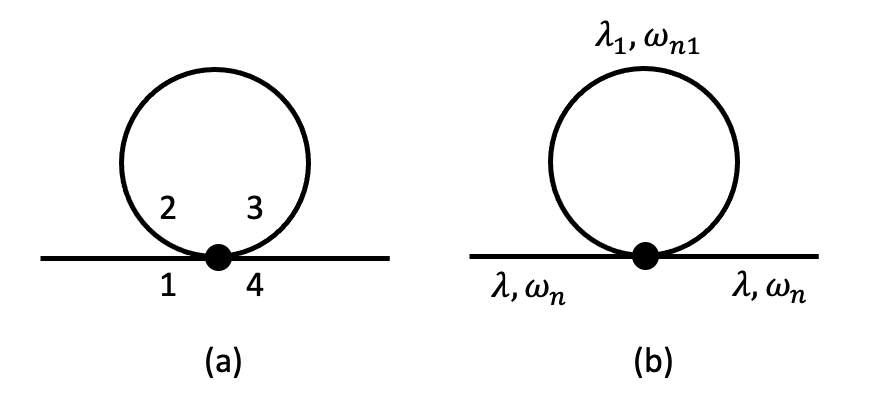
\includegraphics[width=4in]{img/self.energy.1.png}
    \caption{First order in 4-phonon}
    \label{diagram1}
\end{figure}
The factor 12 arise as follows: a single vertex $V^{(4)}$ introduce 4 phonon operator $A_1, A_2, A_3, A_4$, two of them pair
with the external phonon operator and the remaining two pair with themself. 
The number of pairing scheme is thus given by $4\times 3 = 12$.
Calculating Eq.\ref{sigma1} involves evaluating the sum $\sum_{n} G_0(\lambda_1,i\omega_{n})$ with
\begin{equation}
    G_0(\lambda_1,i\omega_{n}) = \frac{1}{\hbar\beta} \left[ \frac{1}{\omega_{\lambda_1}+i\omega_n} + \frac{1}{\omega_{\lambda_1}-i\omega_n} \right]
\end{equation}
Using the technique given in the Appendix A, we have:
\begin{align}
    &\sum_n \frac{1}{\hbar\beta} \left[ \frac{1}{\omega_{\lambda_1}+i\omega_n} + \frac{1}{\omega_{\lambda_1}-i\omega_n} \right] \notag \\
    &= \frac{\beta\hbar}{i} \sum_{p} Res\left[\frac{1}{\hbar\beta} \left[ \frac{1}{\omega_{\lambda_1}+i\omega_p} + \frac{1}{\omega_{\lambda_1}-i\omega_p} \right]\right] n(i\omega_p) \notag \\
    &= -i \sum_{p} Res\left[ \frac{-i}{\omega_p - i\omega_{\lambda_1}} + \frac{i}{\omega_p+i\omega_{\lambda_1}} \right] n(i\omega_p) \notag \\
\end{align}
we have two poles:
\begin{equation}
    Res\left[ \frac{-i}{\omega_p - i\omega_{\lambda_1}} + \frac{i}{\omega_p+i\omega_{\lambda_1}} \right] =
    \begin{cases}
        -i, & \omega_p = i\omega_{\lambda_1} \\
        \ i, & \omega_p = -i \omega_{\lambda_1}
    \end{cases}
\end{equation}
this gives:
\begin{align}
    &\sum_n \frac{1}{\hbar\beta} \left[ \frac{1}{\omega_{\lambda_1}+i\omega_n} + \frac{1}{\omega_{\lambda_1}-i\omega_n} \right] \notag \\
    &= -i \left[ -i n(-\omega_{\lambda_1}) + in(\omega_{\lambda_1}) \right] = n(\omega_{\lambda_1}) - n(-\omega_{\lambda_1}) \notag \\
    &= 2n(\omega_{\lambda_1}) + 1
\end{align}
So that the expression for the self-energy is given by:
\begin{equation}
    \Sigma_{qv} = -\frac{12}{\hbar} \sum_{\lambda_1} V^{(4)}(-\lambda,-\lambda_1,\lambda,\lambda_1) \left[ 2n(\omega_{\lambda_1}) + 1 \right]
\end{equation}

\pagebreak
Figure.\ref{diagram2} is the lowerest order diagram that include the $V^{(3)}$. 
Its expression of the self-energy is given by:
\begin{align}
    \Sigma_{qv} &= \frac{1}{\beta\hbar} (-\beta)^2 18 \sum_{\lambda_1,\lambda_2}\sum_{n_1} V^{(3)}(-\lambda,\lambda_1,\lambda_2) V^{(3)}(\lambda,-\lambda_1,-\lambda_2) 
            G_0(\lambda_1,i\omega_{n_1})G_0(\lambda_2,i(\omega_n-\omega_{n_1})) \notag \\ 
           &= \frac{18\beta}{\hbar} \sum_{\lambda_1,\lambda_2}\sum_{n_1} |V^{(3)}(-\lambda,\lambda_1,\lambda_2)|^2 
           G_0(\lambda_1,i\omega_{n_1})G_0(\lambda_2,i(\omega_n-\omega_{n_1})) \notag \label{sigma2}
\end{align}
\begin{figure}[h!]
    \centering
    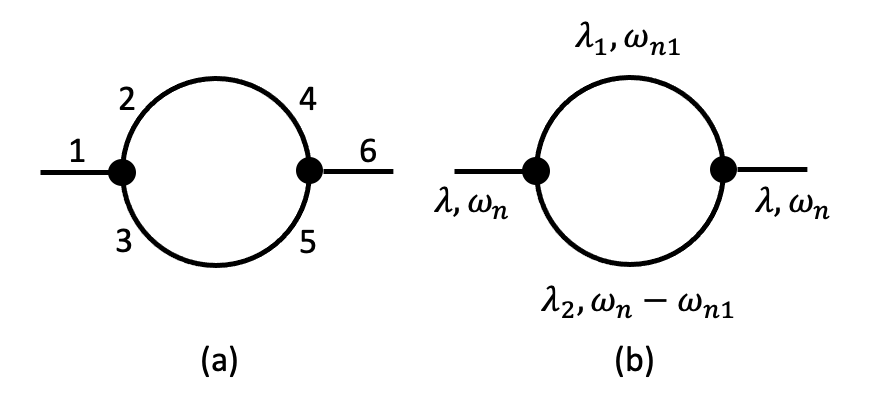
\includegraphics[width=4in]{img/self.energy.2.png}
    \caption{Second order in 3-phonon interaction}
    \label{diagram2}
\end{figure}
where we used $V^{(3)}(-\lambda,\lambda_1,\lambda_2) = V^{(3)}(\lambda,-\lambda_1,-\lambda_2)^*$. The factor 18 comes as follows:
each $V^{(3)}$ brings 3 operator $(1,2,3)$ and $(4,5,6)$, the incoming phonon operator pair with one of the operator from $(1,2,3)$ while 
the out-going phonon operator pair with one from $(4,5,6)$. For the remaining operator, there are two ways to form two pairs. Thus, we have
$3\times 3\times 2 = 18$ different pairing schemes.
The Matsubara sum is evaluated as:
\begin{align}
    &\sum_{n_1} G_0(\lambda_1,i\omega_{n_1})G_0(\lambda_2,i(\omega_n-\omega_{n_1})) \notag \\
    &= \sum_{n_1} \left(\frac{1}{\beta\hbar}\right)^2  \left[ \frac{1}{\omega_{\lambda_1}+i\omega_n} + \frac{1}{\omega_{\lambda_1}-i\omega_n} \right]
                                                       \left[ \frac{1}{\omega_{\lambda_2}+i(\omega_n-\omega_{n_1})} + \frac{1}{\omega_{\lambda_2}-i(\omega_n-\omega_{n_1})} \right] \notag \\
    &= \frac{1}{\beta\hbar} \left\{ \frac{n_2-n_1}{\omega_1 - \omega_2 - i\omega_n} + \frac{n_1+n_2+1}{\omega_1 + \omega_2 - i\omega_n} + \frac{n_1+n_2+1}{\omega_1 + \omega_2 + i\omega_n} + \frac{n_2-n_1}{\omega_1 - \omega_2 + i\omega_n} \right\}
\end{align}
we perform analytic continuation: $i\omega_n \to \Omega + i\eta \ (\eta \to 0^+)$, and using:
\begin{equation}
    \lim_{\eta \to 0^+} \frac{1}{\omega+\Omega\pm i\eta} = P(\frac{1}{\omega+\Omega}) \mp i\pi\delta(\omega + \Omega)
\end{equation}
we obtain the real and imaginary part of self-energy as:
\begin{align}
    \Delta(\omega) = \frac{18}{\hbar^2} \sum_{\lambda_1,\lambda_2} & |V^{(3)}(-\lambda,\lambda_1,\lambda_2)|^2 \notag \\
            & \left\{ (n_2-n_1)\left[ P\left(\frac{1}{\omega_1-\omega_2-\omega}\right)  + P\left(\frac{1}{\omega_1-\omega_2+\omega}\right) \right] \right. \notag \\
            &+ \left. (n_2+n_1+1)\left[ P\left(\frac{1}{\omega_1+\omega_2-\omega}\right) + P\left(\frac{1}{\omega_1+\omega_2+\omega}\right) \right] \right\} \\
    \Gamma(\omega) = \frac{18\pi}{\hbar^2} \sum_{\lambda_1,\lambda_2} & |V^{(3)}(-\lambda,\lambda_1,\lambda_2)|^2 \notag \\
            & \left\{ (n_2-n_1)\left[ \delta(\omega_1-\omega_2-\omega)  + \delta(\omega_1-\omega_2+\omega) \right] \right. \notag \\
            &+ \left. (n_2+n_1+1)\left[ \delta(\omega_1+\omega_2-\omega) + \delta(\omega_1+\omega_2+\omega) \right] \right\} 
\end{align}

\pagebreak
Figure.\ref{diagram3} is the second order diagram with $V^{(4)}$, its expression is given by:
\begin{align}
    \Sigma_{qv} &= \frac{96\beta}{\hbar} \sum_{\lambda_1,\lambda_2,\lambda_3}
                \sum_{n_1}\sum_{n_2} |V^{(4)}(-\lambda,\lambda_1,\lambda_2,\lambda_3)|^2  
            G_0(\lambda_1,i\omega_{n_1})G_0(\lambda_2,i\omega_{n_2})G_0(\lambda_3,i(\omega_n-\omega_{n_1}))  \label{sigma3}
\end{align}
\begin{figure}[h!]
    \centering
    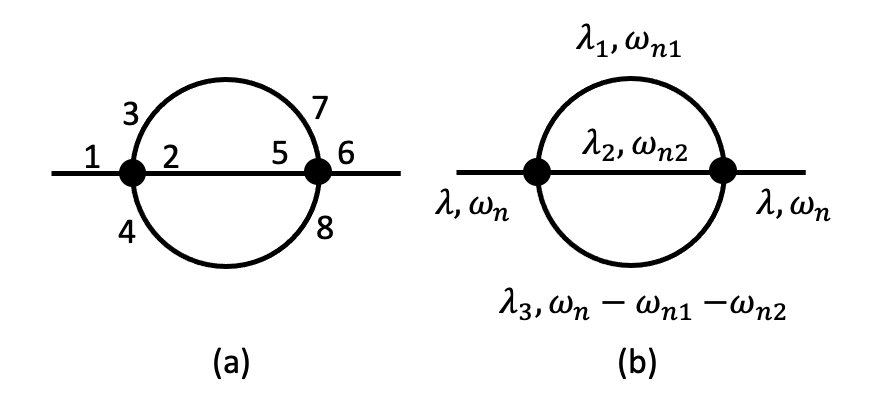
\includegraphics[width=4in]{img/self.energy.3.png}
    \caption{Second order in 4-phonon interaction}
    \label{diagram3}
\end{figure}
where now the factor 96 is counted similar as in the case of Eq.\ref{sigma2} but now each vertex provide 4 different operators. We have 
the pairing scheme: $4\times 4\times 6 = 96$, where 6 comes from the pairing between 6 operators.
We present the result of evaluating Matsubara sum below. For the real part, we have:
\begin{align}
    \Delta(\omega) = & \frac{96}{\hbar^2} \sum_{\lambda_1,\lambda_2,\lambda_3}  |V^{(4)}(-\lambda,\lambda_1,\lambda_2,\lambda_3)|^2  \notag \\
            & \left\{ \left[ (n_1+1)(n_2+1)(n_3+1) - n_1n_2n_3 \right] P\left(\frac{1}{\omega-\omega_1-\omega_2-\omega_3} - \frac{1}{\omega+\omega_1+\omega_2+\omega_3}\right) \right. \notag \\
            &+ \left. 3 \left[ n_1(n_2+1)(n_3+1) - (n_1+1)n_2n_3 \right] P\left(\frac{1}{\omega+\omega_1-\omega_2-\omega_3} - \frac{1}{\omega-\omega_1+\omega_2+\omega_3}\right) \right\}  
\end{align}
and the imaginary part:
\begin{align}
    \Gamma(\omega) = & \frac{96\pi}{\hbar^2} \sum_{\lambda_1,\lambda_2,\lambda_3}  |V^{(4)}(-\lambda,\lambda_1,\lambda_2,\lambda_3)|^2  \notag \\
            & \left\{ \left[ (n_1+1)(n_2+1)(n_3+1) - n_1n_2n_3 \right] \left(\delta(\omega-\omega_1-\omega_2-\omega_3) - \delta(\omega+\omega_1+\omega_2+\omega_3) \right) \right.  \notag \\
            &+ \left. 3 \left[ n_1(n_2+1)(n_3+1) - (n_1+1)n_2n_3 \right] \left(\delta(\omega+\omega_1-\omega_2-\omega_3) - \delta(\omega-\omega_1+\omega_2+\omega_3) \right)  \right\}  
\end{align}

\pagebreak
\section*{Appendix A}
\subsection*{Evaluating the Matsubara Sum}
Evaluating Matsubara sum involve calculating:
\begin{equation}
    \sum_n f(i\omega_n) \notag
\end{equation}
Suppose we have an integral,
\begin{equation}
    \int_c f(i\omega) n(i\omega) d(i\omega) \notag
\end{equation}
where curve $c$ cover all the singularity of the function $f(i\omega)$ and $n(i\omega)$.
If $f(i\omega) \to 0$ at infinity, the integral will vanish:
\begin{equation}
    \int_c f(i\omega) n(i\omega) d(i\omega) = \sum_n Res[n(i\omega_n)] f(i\omega_n) + \sum_p Res[f(i\omega_p)] n(i\omega_p) = 0 \notag
\end{equation}
where the summation run through the poles of function $n(i\omega)$ and $f(i\omega)$. 
If we take $n(i\omega)$ to be the Bose-Einstein distribution function, we have:
\begin{gather}
    n(\omega) = \frac{1}{e^{\beta\hbar\omega} - 1} \notag \\
    n(i\omega) = \frac{1}{e^{i\beta\hbar\omega} - 1} \notag
\end{gather}
$n(i\omega)$ has poles at $\omega_n = \frac{2\pi n}{\beta\hbar}$, the residual of $n(i\omega)$ at those poles 
are: $Res[n(i\omega_n)] = -i/\beta\hbar$. We have the result:
\begin{equation}
    \sum_n f(i\omega_n) = \frac{\beta\hbar}{i} \sum_{p} Res[f(i\omega_p)] n(i\omega_p)
\end{equation}
so that we need to sum over all the residuals in the function $f(i\omega)$.

\pagebreak
\section*{Appendix B}
\subsection*{Non-interacting Green's function}
We write the bare Green's function as:
\begin{align}
    G_0(qv;\tau) = 
    \begin{cases}
        \frac{1}{Z} Tr\left\{ e^{-(\beta-\tau/\hbar)H_0} A_{qv} e^{-\tau/\hbar H_0} A_{qv}^{\dagger} \right\}, &\tau > 0 \\
        \frac{1}{Z} Tr\left\{ e^{-\beta H_0} A_{qv}^{\dagger} e^{\tau/\hbar H_0} A_{qv} e^{- \tau/\hbar H_0} \right\}, &\tau < 0 \\
    \end{cases}
\end{align}
We first consider the case when $\tau > 0$, by inserting the set of eigenstate $\sum_j |j\rangle \langle j | $, we have
\begin{align}
    G_0(qv;\tau) &= \frac{1}{Z} \sum_i \sum_j e^{-\beta \varepsilon_i} \langle i | e^{\tau H_0/\hbar} (a_{qv} + q_{-qv}^{\dagger}) e^{-\tau H_0/\hbar} | j \rangle 
                        \langle j | (a_{qv}^{\dagger} + q_{-qv}) | i \rangle  \notag \\
                &= \frac{1}{Z} \sum_i \sum_j e^{-\beta \varepsilon_i} e^{\tau(\varepsilon_i - \varepsilon_j)/\hbar} 
                \langle i | (a_{qv} + q_{-qv}^{\dagger}) | j \rangle \langle j | (a_{qv}^{\dagger} + q_{-qv}) | i \rangle  \notag \\
                &= e^{\tau \omega_q} \langle n_q \rangle + e^{- \tau \omega_q}  \langle n_q  + 1\rangle \notag \\
                &= \frac{e^{\tau \omega_q}}{e^{\beta \hbar \omega_q} - 1} + \frac{e^{-\tau \omega_q}}{1 - e^{-\beta \hbar \omega_q} }
\end{align}
where we used:
\begin{align}
    a | n \rangle &= \sqrt{n} | n-1 \rangle  \notag \\
    a^{\dagger} | n \rangle &= \sqrt{n+1} | n+1 \rangle \notag \\
\end{align}
for the case when $\tau > 0$, we follow the same procedure to obtain:
\begin{align}
    G_0(qv;\tau) &= \frac{1}{Z} \sum_i \sum_j e^{-\beta \varepsilon_i} \langle i | (a_{qv}^{\dagger} + q_{-qv}) | j \rangle
                        \langle j | e^{\tau H_0/\hbar} (a_{qv} + q_{-qv}^{\dagger}) e^{-\tau H_0/\hbar} | i \rangle  \notag \\
                &= e^{\tau \omega_q} \langle n_q + 1\rangle + e^{- \tau \omega_q} \langle n_q \rangle \notag \\
                &= \frac{e^{- \tau \omega_q}}{e^{\beta \hbar \omega_q} - 1} + \frac{e^{\tau \omega_q}}{1 - e^{-\beta \hbar \omega_q} }
\end{align}
therefore, the phonon green's function can be written as:
\begin{equation}
    G_0(qv;\tau) = \frac{e^{|\tau| \omega_q}}{e^{\beta \hbar \omega_q} - 1} + \frac{e^{-|\tau| \omega_q}}{1 - e^{-\beta \hbar \omega_q} }
\end{equation}
which is an even function.

\pagebreak
\section*{Appendix C}
\subsection*{Deriving the diagramatic rules}
Our task is to evaluate the expression for $G(qvv';\tau)$ as:
\begin{align}
    G(qvv';\tau)= \sum_{n=0}^{\infty} \frac{1}{n!} \left( -\frac{1}{\hbar} \right)^{n} 
    \int_0^{\beta\hbar} d\tau_1 \cdots \int_0^{\beta\hbar} d\tau_{n} \left\langle \mathcal{T}[ A_{qv}(\tau) A_{qv'}^{\dagger}(0) H_I(\tau_1) \cdots H_I(\tau_{n}) ] \right\rangle_{0,c} 
\end{align}
we consider the case of first order perturbation from four-phonon interaction, which correspond to Figure.\ref{diagram1}. Now the 
expression is simply:
\begin{align}
    G(q;\tau)&= \left( -\frac{1}{\hbar} \right) 
    \int_0^{\beta\hbar} d\tau_1 \left\langle \mathcal{T}\left[ A_{q}(\tau) A_{q}^{\dagger}(0) \sum_{q_{1\cdots 4}}V(q_1,q_2,q_3,q_4) A_{q_1}(\tau_1)A_{q_2}(\tau_1)A_{q_3}(\tau_1)A_{q_4}(\tau_1)\right] \right\rangle_{0,c} \notag \\
    &= -\frac{12}{\hbar}  
    \sum_{q_1} V(-q,q,-q_1,q_1) \int_0^{\beta\hbar} d\tau_1 \left\langle \mathcal{T}[ A_q(\tau_1)A_{q}^{\dagger}(0) ] \right\rangle
    \left\langle \mathcal{T}[ A_{q}(\tau)A_{q}^{\dagger}(\tau_1) ] \right\rangle 
    \left\langle \mathcal{T}[ A_{q_1}(\tau_1)A_{q_1}^{\dagger}(\tau_1) ] \right\rangle \notag \\
    &= -\frac{12}{\hbar} \sum_{q_1} V(-q,q,-q_1,q_1) \int_0^{\beta\hbar} d\tau_1 G_0(q;\tau_1) G_0(q;\tau-\tau_1) G_0(q_1;0) \notag \\
    &= -\frac{12}{\hbar} \sum_{q_1} V(-q,q,-q_1,q_1) \int_0^{\beta\hbar} d\tau_1 
        \sum_{n_1}G_0(q;i\omega_{n_1}) e^{i\omega_{n_1}\tau_1} 
        \sum_{n_2}G_0(q;i\omega_{n_2}) e^{i\omega_{n_2}(\tau-\tau_1)} 
        \sum_{n_3}G_0(q_1;i\omega_{n_3}) \notag \\
    &= -\frac{12}{\hbar} \sum_{q_1} V(-q,q,-q_1,q_1) \sum_{n_1,n_2} G_0(q;i\omega_{n_1}) G_0(q;i\omega_{n_2}) e^{i\omega_{n_2}\tau} 
        \int_0^{\beta\hbar} d\tau_1 e^{i(\omega_{n_1}-\omega_{n_2})\tau_1} \sum_{n_3}G_0(q_1;i\omega_{n_3}) \notag \\
    &= -12\beta \sum_{q_1} V(-q,q,-q_1,q_1) \sum_{n_1} G_0(q;i\omega_{n_1}) G_0(q;i\omega_{n_1}) e^{i\omega_{n_1}\tau} 
        \sum_{n_3}G_0(q_1;i\omega_{n_3})
\end{align}
where the thermal average is contracted into pairs with Wick's theorem at finite temperature and we used the fact that
\begin{equation}
    \int_0^{\beta\hbar} d\tau_1 e^{i(\omega_{n_1}-\omega_{n_2})\tau_1} = \beta\hbar \delta_{n_1,n_2}
\end{equation}.
To see how it give raise to self-energy, we perform transformation into frequency space:
\begin{align}
    G(q;i\omega_n) &= \frac{1}{\beta\hbar} \int_{0}^{\beta\hbar} G(q;\tau) e^{-i\omega_n\tau} d\tau \notag \\
        &= -\frac{12}{\hbar}\sum_{q_1} V(-q,q,-q_1,q_1) 
        \int_{0}^{\beta\hbar} \sum_{n_1} G_0(q;i\omega_{n_1}) G_0(q;i\omega_{n_1}) e^{i(\omega_{n_1}-\omega_n)\tau}  d\tau
        \sum_{n_3}G_0(q_1;i\omega_{n_3})  \notag \\
        &= -12\beta \sum_{q_1} V(-q,q,-q_1,q_1) G_0(q;i\omega_{n}) G_0(q;i\omega_{n})
        \sum_{n_3}G_0(q_1;i\omega_{n_3}) 
\end{align}
The self-energy is defined to be:
\begin{equation}
    G(q;i\omega_n) = G_0(q;i\omega_n) + \frac{1}{\beta\hbar} G_0(q;i\omega_n) \Sigma(q;i\omega_n) G(q;i\omega_n)
\end{equation}
so that we find the self-energy in the above expression:
\begin{equation}
    \Sigma^{(4)}(q;i\omega_n) = -\frac{12}{\hbar} \sum_{q_1} V(-q,q,-q_1,q_1) \sum_{n_1}G_0(q_1;i\omega_{n_1}) 
\end{equation}
\subsection*{General case}
In the general case, we can establish the rules as follow for the expression of phonon Green's function:
\begin{align}
    G(qvv';\tau)= \sum_{n=0}^{\infty} \frac{1}{n!} \left( -\frac{1}{\hbar} \right)^{n} 
    \int_0^{\beta\hbar} d\tau_1 \cdots \int_0^{\beta\hbar} d\tau_{n} \left\langle \mathcal{T}[ A_{qv}(\tau) A_{qv'}^{\dagger}(0) H_I(\tau_1) \cdots H_I(\tau_{n}) ] \right\rangle_{0,c} 
\end{align}
\begin{enumerate}
    \item Factor $1/n!$ is cancelled with the $n!$ permutation of internal time coordinates.
    \item Carry out all integral with respect to internal time give a factor $(\beta\hbar)^n$ .
    \item Finding the number of pairing scheme in the Wick theorem expansion.
\end{enumerate}
Therefore, the remaining factor is only $(-\beta)^n$. There is an additional definition of 
$\frac{1}{\beta\hbar}$ in the self-energy, Therefore, the rules for evaluating self-energy 
is 
\begin{enumerate}
    \item Overall factor of $\frac{1}{\beta\hbar} (-\beta)^n$, where $n$ is the number of the vertexes.
    \item Multiply the number of ways to pair the phonon modes.
    \item Multiply appropriate $V$ for each vertex.
    \item For each internal line, multiply $G_0(qvv';i\omega^i_n)$.
    \item Sum over all internal coordinates $q^i;v^i$ and Matsubara frequency $\omega_n^i$
\end{enumerate}

\pagebreak
\section*{Appendix D. Wick's theorem at finite temperature}
Evaluating the perturbation expansion involves calculating the thermal average on $N$ operators with  
non-perturbed Hamiltonian $H_0$, where
$N$ must be a even number so that the result is non-zero:
\begin{equation}
    \text{Tr}\left[ \rho_o ABC \cdots XYZ  \right]
\end{equation}
with 
\begin{equation}
    \text{Tr}\left[ \rho_o \mathcal{A} \right] = \sum_i \langle i | e^{\beta(\Omega_0 - H_0 + \mu N)} \mathcal{A} |i \rangle
\end{equation}

\subsection*{Fermion}
we first consider of case of fermions, we use the anticommunication relationship
of fermion creation and annihilation operator: $\{ a_k^{\dagger} , a_{k'} \} = \delta_{kk'}$ to 
exchange the order of operator in the average:
\begin{align}
    &\text{Tr}\left[ \rho_o ABC \cdots XYZ  \right] \notag \\
    = &\text{Tr}\left[ \rho_o \{A,B\} C \cdots XYZ  \right] - \text{Tr}\left[ \rho_o BAC \cdots XYZ  \right] \notag \\
    = &\text{Tr}\left[ \rho_o \{A,B\} C \cdots XYZ  \right] - \left( \text{Tr}\left[ \rho_o B\{A,C\} \cdots XYZ  \right] - \text{Tr}\left[ \rho_o BCA \cdots XYZ  \right] \right) \notag \\
    = &\text{Tr}\left[ \rho_o \{A,B\} C \cdots XYZ  \right] - \text{Tr}\left[ \rho_o B\{A,C\} \cdots XYZ  \right] \notag \\
    & + \cdots + \text{Tr}\left[ \rho_o BC \cdots XY\{A,Z\}  \right] - \text{Tr}\left[ \rho_o BC \cdots XYZA  \right] \label{contraction1}
\end{align}
As an example, 
\begin{align}
    \text{Tr}\left[ \rho_o ABCD  \right] = \text{Tr}\left[ \rho_o\{A,B\} CD \right] - \text{Tr}\left[ \rho_o B\{A,C\} D \right] + \text{Tr}\left[ \rho_o BC\{A,D\} \right] - \text{Tr}\left[ \rho_o BCDA \right]
\end{align}
The sign of each term containing an anticommunicator is given by $(-1)^{n-1}$, the number $n$ of exchange done. For the final term, its sign
is given by the sign of last term that contain an anticommunicator multiplied by $-1$, which will always be negative because we perform maximum
$N-1$ exchange and N is a even number. 

Now, we can verify that:
\begin{align}
    \langle j | a_k^{\dagger} e^{\beta(\Omega_0 - H_0 + \mu N)} | i \rangle 
            &= e^{\beta(\Omega_0 - E_i + \mu N_i)} \langle j |a_k^{\dagger} | i \rangle  \notag \\
    \langle j | e^{\beta(\Omega_0 - H_0 + \mu N)} a_k^{\dagger}  | i \rangle 
            &= e^{\beta(\Omega_0 - E_j + \mu N_j)} \langle j |a_k^{\dagger} | i \rangle  \notag \\
            &= e^{\beta(\Omega_0 - (E_i+\varepsilon_k) + \mu (N_i+1))} \langle j |a_k^{\dagger} | i \rangle  \notag \\
            &= e^{-\beta (\varepsilon_k - \mu)} \langle j | a_k^{\dagger} e^{\beta(\Omega_0 - H_0 + \mu N)} | i \rangle \label{rhoA}
\end{align}
so that 
\begin{equation}
    \rho_0 a_k^{\dagger} = e^{-\beta (\varepsilon_k - \mu)} a_k^{\dagger} \rho_0
\end{equation}
as well as the relation:
\begin{equation}
    \rho_0 a_k = e^{\beta (\varepsilon_k - \mu)} a_k \rho_0
\end{equation}
So that we can conclude
\begin{equation}
    A\rho_0 = e^{\lambda_A \beta (\varepsilon_k - \mu)} \rho_0 A\ \ \
    \begin{cases}
        \lambda_A = 1 , & A = a_k^{\dagger} \\
        \lambda_A = -1 , & A = a_k \\
    \end{cases}
\end{equation}
and 
\begin{align}
    \text{Tr}\left[ \rho_o BC \cdots XYZA  \right] &= \text{Tr}\left[ A \rho_o BC \cdots XYZ  \right] \notag \\
                            &= e^{\lambda_A \beta (\varepsilon_k - \mu)} \text{Tr}\left[ \rho_o ABC \cdots XYZ  \right] \notag \\
\end{align}
Since for fermion operators, their anticommunicator is a C-number, 
Eq.\ref{contraction1} becomes:
\begin{align}
    \text{Tr}\left[ \rho_o ABC \cdots XYZ  \right] &= \frac{\{A,B\}}{e^{\lambda_A \beta (\varepsilon_k - \mu)} + 1} \text{Tr}\left[ \rho_o C \cdots XYZ  \right] \notag \\
                                                & - \frac{\{A,C\}}{e^{\lambda_A \beta (\varepsilon_k - \mu)} + 1} \text{Tr}\left[ \rho_o BD \cdots XYZ  \right] \notag \\
                                                & + \cdots +  (-1)^{n-1} \frac{\{A,Z\}}{e^{\lambda_A \beta (\varepsilon_k - \mu)} + 1} \text{Tr}\left[ \rho_o BC \cdots XY  \right] \label{contraction2}
\end{align}
where $n$ is the number of exchanges of operator needed. 

Next, we calculate the term:
\begin{equation}
    \frac{\{A,B\}}{e^{\lambda_A \beta (\varepsilon_k - \mu)} + 1}
\end{equation}
\textbf{case 1} we let $A = a_k^{\dagger}$, so that $B = a_k$. we have:
\begin{align}
    \frac{\{a_k^{\dagger},a_k\}}{e^{ \beta (\varepsilon_k - \mu)} + 1} = \frac{1}{e^{\beta (\varepsilon_k - \mu)} + 1} = \langle a_k^{\dagger} a_k \rangle = \langle AB \rangle
\end{align}
\textbf{case 2} we let $A = a_k$, so that $B = a_k^{\dagger}$. we have:
\begin{align}
    \frac{\{a_k,a_k^{\dagger}\}}{e^{-\beta (\varepsilon_k - \mu)} + 1} = \frac{1}{e^{ -\beta (\varepsilon_k - \mu)} + 1} = \langle a_k a_k^{\dagger} \rangle = \langle AB \rangle
\end{align}
So that in both case, we have the relationship:
\begin{equation}
    \frac{\{A,B\}}{e^{\lambda_A \beta (\varepsilon_k - \mu)} + 1} = \langle AB \rangle
\end{equation}
and Eq.\ref{contraction2} can now be written:
\begin{align}
    \langle ABC \cdots XYZ  \rangle = & \langle AB  \rangle \langle  C \cdots XYZ \rangle  - \langle AC\rangle  \langle BD \cdots XYZ  \rangle  \notag \\
                                                & + \cdots + (-1)^{n-1} \langle AZ\rangle  \langle BC \cdots XY  \rangle \label{wick1}
\end{align}

Thus we have factorized out all the pairs of operators that contain $A$, the process can continue until the initial thermal average is completely written
as the sum of product of averages of pairs, the sign of which is determined by the number of exchanges to arrive at the specific pairing.

\subsection*{Boson}
Instead of the anticommunicator, we use communicator of boson operators:
\begin{gather}
    [ b_q^{\dagger} , b_{q'} ] = - \delta_{qq'} \notag \\  
    [ b_{q}, b_{q'}^{\dagger} ] = \delta_{qq'}  \notag
\end{gather}
so that Eq.\ref{contraction1} becomes:
\begin{align}
    &\text{Tr}\left[ \rho_o ABC \cdots XYZ  \right] \notag \\
    = &\text{Tr}\left[ \rho_o [A,B] C \cdots XYZ  \right] + \text{Tr}\left[ \rho_o BAC \cdots XYZ  \right] = \cdots \notag \\
    = &\text{Tr}\left[ \rho_o [A,B] C \cdots XYZ  \right] + \text{Tr}\left[ \rho_o B[A,C] \cdots XYZ  \right] \notag \\
    & + \cdots + \text{Tr}\left[ \rho_o BC \cdots XY[A,Z]  \right] + \text{Tr}\left[ \rho_o BC \cdots XYZA  \right] \label{contractionq1}
\end{align}
The relation Eq.\ref{rhoA} still holds, so that:
\begin{align}
    \text{Tr}\left[ \rho_o ABC \cdots XYZ  \right] &= \frac{[A,B]}{1 - e^{\lambda_A \beta (\varepsilon_q - \mu)} } \text{Tr}\left[ \rho_o C \cdots XYZ  \right] \notag \\
                                                & + \frac{[A,C]}{1 - e^{\lambda_A \beta (\varepsilon_q - \mu)} } \text{Tr}\left[ \rho_o BD \cdots XYZ  \right] \notag \\
                                                & + \cdots + \frac{[A,Z]}{1 - e^{\lambda_A \beta (\varepsilon_q - \mu)} } \text{Tr}\left[ \rho_o BC \cdots XY  \right] \label{contractionq2}
\end{align}
For bosons, we can find:
\begin{align}
    \frac{[b_q^{\dagger},b_q]}{1 - e^{ \beta (\varepsilon_q - \mu)} } &= \frac{-1}{1 - e^{\beta (\varepsilon_q - \mu)} } 
        = \langle n_q \rangle = \langle b_q^{\dagger} b_q \rangle  \notag \\
    \frac{[b_q,b_q^{\dagger}]}{1 - e^{ -\beta (\varepsilon_q - \mu)} } &= \frac{1}{1 - e^{-\beta (\varepsilon_q - \mu)} } 
        = \langle n_q + 1\rangle = \langle b_q b_q^{\dagger} \rangle  \notag \\
\end{align}
as a result 
\begin{equation}
    \frac{[A,B]}{1 - e^{ \beta (\varepsilon_q - \mu)} } = \langle AB \rangle 
\end{equation}
and the analogy of Eq.\ref{wick1} for bosons are therefore:
\begin{align}
    \langle ABC \cdots XYZ  \rangle = & \langle AB  \rangle \langle  C \cdots XYZ \rangle  + \langle AC\rangle  \langle BD \cdots XYZ  \rangle  \notag \\
                                                & + \cdots + \langle AZ\rangle  \langle BC \cdots XY  \rangle \label{wick2}
\end{align}

\end{document}